\documentclass{scrbook}

\usepackage{natbib}
\usepackage{graphicx}
\usepackage{amsthm}
\usepackage{amsmath}

\linespread{1.5}

\title{Demonstrating Quantum Speed-Up with a 2 Transmon Quantum Processor.}
\author{Andreas Dewes}

\theoremstyle{definition}
\newtheorem{theorem}{Theorem}[chapter]
\newtheorem{axiom}{Axiom}[theorem]

\newcommand{\ket}[1]{\left| #1 \right>} % for Dirac bras
\newcommand{\bra}[1]{\left< #1 \right|} % for Dirac kets

\begin{document}

\maketitle

\tableofcontents

\listoffigures

\listoftables

\chapter{Introduction}

%-General introduction in the research field: Quantum mechanics, superposition, entanglement

\section{Quantum Computing}

%-Discuss the interest of quantum computation and possible paradigms: Classical, surface-code, topological...

\section{Superconducting Quantum Bits}

%-Discuss types of superconducting quantum bits (flux, phase, charge, hybrid)

\section{Circuit Quantum Electrodynamics}

%-Discuss CQED as the architecture used throughout this work.


%-A 2-Qubit Quantum Processor
%-Building Blocks: Single Qubit Gates, Qubit Readout, 2-Qubit Gate
%-Implementation
%-Frequency Tunability of the Qubits
%  -Decoherence Times
%-Characterization of the Readout
%  -Readout Errors
%-Single Qubit Gates: Tune-Up & Characterization
%-2 Qubit Gate: Tune-Up & Characterization
%-Tests of Entanglement
%  -Entanglement Witnesses
%  -Bell's Inequality
%-2 Qubit Algorithms
%-Grover's Search Algorithm:
%   -Introduction & Background
%   -Implementation
%   -Measurements
%   -Error Analysis
%   -Conclusions

\chapter{Experiments}

%-Discuss all the experiments performed during the PhD thesis.

\section{Realizing a 2-Qubit Quantum Processor}

%-Motivate the performed experiments.

\begin{figure}
	\centering	
	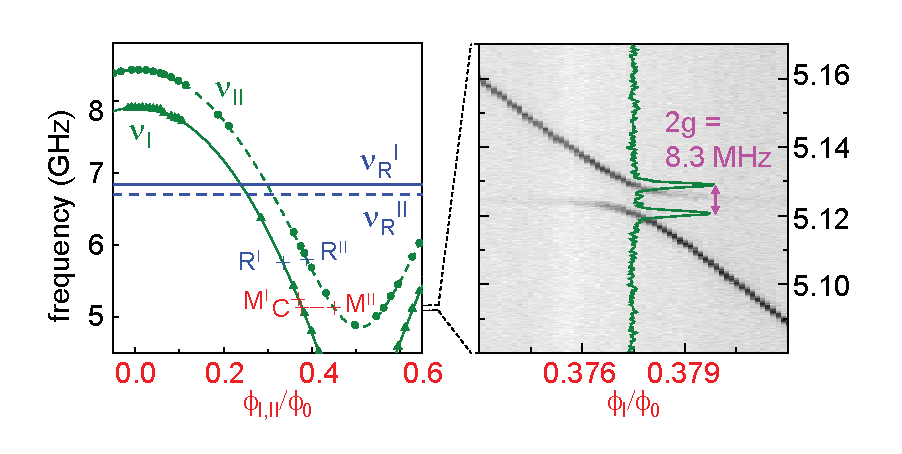
\includegraphics[width=0.8\textwidth]{./material/papers/iswap/figures/2_qubit_processor_spectrocopy}
	\label{fig:ProcessorSpectroscopy}
	\caption{}
\end{figure}

\subsection{Requirements}

%-List requirements for diVincenzo-style quantum computation:
%-Good 1 & 2 Qubit Gates
%-Qubits can be reset
%-Individual Single Shot Readout with High Fidelity

\subsection{Design \& Implementation}

%-Discuss the design & realization of our 2-qubit processor:
%  -Chip design
%  -Analytical model and parameter design.
%  -Measurement setup & RF chain

\section{Characterization of the Processor}

%-Show basic characteristics of the processor:
%  -Qubit transition energies vs. fluxes
%  -Qubit fast frequency controls
%  -2 Qubit interaction

\subsection{Readout}

%-Discuss the readout errors and crosstalk

\subsection{Single-Qubit Manipulation}

%-Discuss single qubit manipulation, gate fidelity and state tomography
%Data: 14/12/2010

\subsection{Implementing an Universal 2-Qubit Gate: $\sqrt{i\mathrm{SWAP}}$}

\begin{figure}
	\centering
		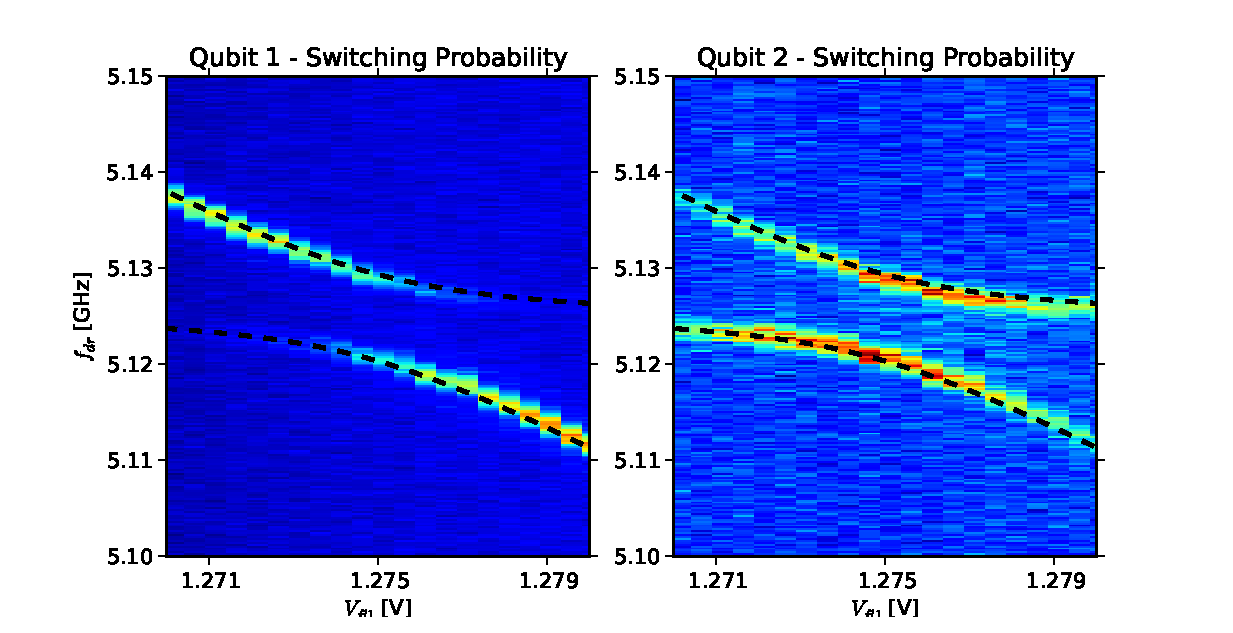
\includegraphics[width=1.\textwidth]{./material/figures/2-qubit-processor/characterization/anticrossing/anticrossing}
	\label{fig:QubitAnticrossing}
	\caption{}
\end{figure}


\begin{figure}
	\centering
		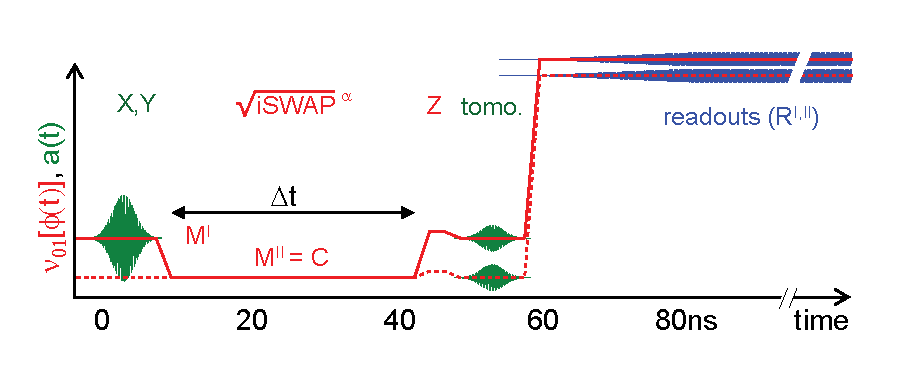
\includegraphics[width=0.8\textwidth]{./material/papers/iswap/figures/iswap_gate_pulse_sequence}
	\label{fig:ISwapPulseSequence}
	\caption{}
\end{figure}


%-Discuss the realization of a 2 qubit gate:
%  -Principle
%  -Implementation & Pulse Sequency
%  -Characterization through Quantum Process Tomography:
%     -Principles: State tomography, Pauli set, process tomography
%     -Discuss alternative representations of the process information:
%        -Chi matrix, Choi matrix, S, log S, Kraus operator representation
%  		-Errors: Discuss simulations, error models and possible reasons for discrepancies

%-Discuss the generation of Bell states, the measurement of entanglement witnesses and the measured violation of the CHSH equation.


%To Do:
% -Look through the swapping data and see if there's evidence for wavefunction collapse in qubit 2 when qubit 1 is measured and the two qubits are only partially entangled. Compare the Leo's proposition.

\subsection{Violation of Bell's inequality}

\begin{figure}
	\centering
		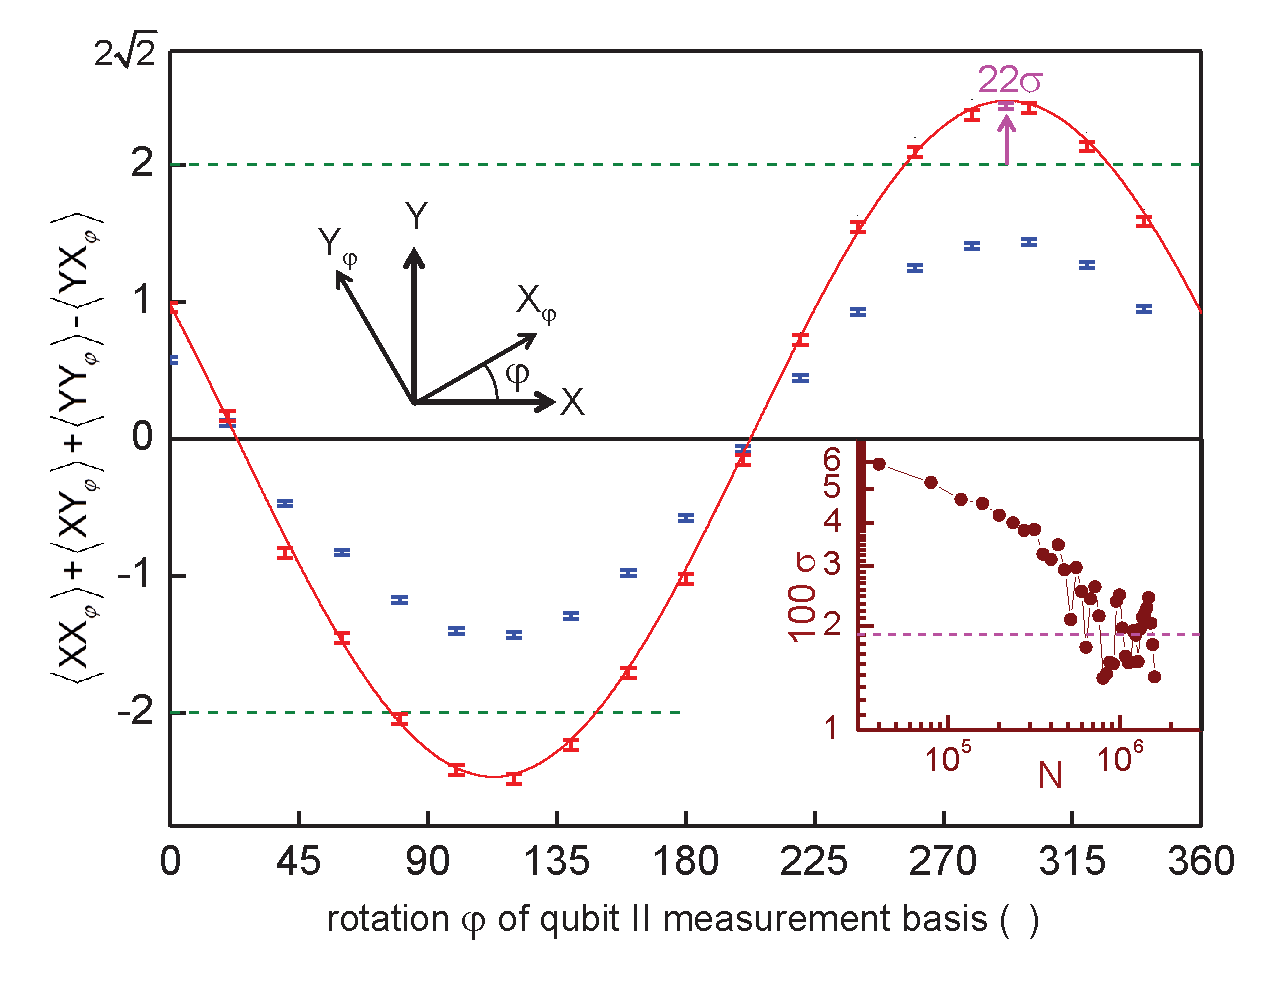
\includegraphics[width=0.8\textwidth]{./material/papers/iswap/figures/chsh}
	\label{fig:CHSH}
	\caption{}
\end{figure}

\subsection{Quantum State Tomography}

Quantum state tomography is the procedure of experimentally determining an unknown quantum state\cite{michael_a._nielsen_quantum_2000}.

\begin{eqnarray}
\rho & = & \sum\limits_{v_1,v_2\hdots v_n} \frac{c_{v_1,v_2\hdots v_n} \sigma_{v_1}\otimes \sigma_{v_2}\hdots \sigma_{v_n}}{2^n} \label{eq:state_tomography_state_representation} \\
c_{v_1,v_2\hdots v_n} & = & \mathrm{tr}\left(\sigma_{v_1}\otimes \sigma_{v_2}\hdots \sigma_{v_n} \; \rho \right)  \label{eq:state_tomography_coefficients}
\end{eqnarray}

where $v_i \in \left\{ X,Y,Z,I\right\}$ and $n$ gives the number of qubits in the system. To determine the coefficients $c_{v_1,v_2\hdots v_n}$ we prepare an ensemble of identical states $\rho$ and measure the expectation value of the operator $\sigma_{v_1}\otimes \sigma_{v_2}\hdots \sigma_{v_n}$. However, this would involve measuring the expectation values of the operators $\sigma_{X}$ and $\sigma_{Y}$, which we cannot do in experiment. Therefore, instead of directly measuring $\sigma_x$ or $\sigma_y$, we perform a rotation $\Theta_{\pi /2}(Y)$ or $\Theta_{-\pi /2}(X)$ first and measure $\sigma_z$ afterwards, which yields the same result. \todo{check the signs of the rotations!}

Repeating this method many times and averaging the result then gives an estimate of the coefficients $c_{v_1,v_2\hdots v_n}$. Unfortunately, when estimating these coefficients one-by-one, small measurement and preparation errors can yield a density matrix $\rho$ which is {\it non-physical} i.e. which violates the positivity or unity-trace properties of a physical density matrix. There, often we use techniques for jointly estimating all $c_{v_1,v_2\hdots v_n}$'s within the set of acceptable density matrices.

\subsubsection{Maximum Likelihood Estimation}

A method which is often used in quantum state tomography is the so-called {\it maximum-likelihood} technique, which works in the following way:

\subsection{Process Tomography of the Quantum Gate}

A quantum process can be described as a map $\mathcal{E} : \rho_\mathcal{H} \to \rho_\mathcal{H}$ that maps a density matrix $\rho$ defined in a Hilbert space $Q_1$ to another density matrix $\mathcal{E}(\rho)$ defined in a target Hilbert space $Q_2$ and fulfilling three axiomatic properties \cite{michael_a._nielsen_quantum_2000,haroche_exploring_2006}:

\begin{axiom}
$\mathrm{tr}\left[\mathcal{E}(\rho)\right]$ is the probability that the process represented by $\mathcal{E}$ occurs, when $\rho$ is the initial state.
\end{axiom}

\begin{axiom}
$\mathcal{E}$ is a {\it convex-linear map} on the set of density matrices, that is, for probabilities $\left\{p_i\right\}$,

  \begin{equation}
	  \mathcal{E}\left(\sum\limits_i p_i \rho_i\right) = \sum\limits_i p_i \mathcal{E}(\rho_i)
	\end{equation}
\end{axiom}

\begin{axiom}
$\mathcal{E}$ is a {\it completely-positive} map. That is, if $\mathcal{E}$  maps density operators of system $Q_1$ to density operators of system $Q_2$, then $\mathcal{E}(A)$ must be positive for any positive operator $A$. Furthermore, if we introduce an extra system $R$ of arbitrary dimensionality, it must be true that $(\mathcal{I}\otimes \mathcal{E})(A)$ is positive for any positive operator $A$ on the combined system $RQ_1$, where $\mathcal{I}$ denotes the identity map on system $R$.
\end{axiom}
As shown in \cite{michael_a._nielsen_quantum_2000}, any quantum process fulfilling these criteria can be written in the form

\begin{equation}
  \mathcal{E}(\rho) = \sum\limits_i E_i \rho E_i^\dagger \label{eq:process_operator_sum_representation}
\end{equation}
for some set of operators $\{ E_i \}$ which map the input Hilbert space to the output Hilbert space, and $\sum_i E_i^\dagger E_i \le I$.

Now, if we express the operators $E_i$ in a different operator basis $\tilde{E}_j$ such that $E_i = \sum_j a_{ij} \tilde{E}_{j}$ and insert into eq. (\ref{eq:process_operator_sum_representation}), we obtain

\begin{eqnarray}
 \mathcal{E}(\rho) & = & \sum\limits_i \sum\limits_j a_{ij} \tilde{E}_j \;\rho\; \sum\limits_k a_{ik}^* \tilde{E}_k^\dagger \\
& = & \sum\limits_{j,k}\tilde{E}_j \; \rho \; \tilde{E}_k^\dagger \sum\limits_i a_{ij} a_{ik}^* \\
& = & \sum\limits_{j,k}\tilde{E}_j \; \rho \; \tilde{E}_k^\dagger \; \chi_{jk} \label{eq:process_chi_representation}
\end{eqnarray}
where we defined $\chi_{jk} = \sum\limits_i a_{ij} a_{ik}^*$. This is the so-called $\chi$-matrix representation of the quantum process. Here, all the information on the process is contained in the $\chi$ matrix, which controls the action of the process-independent operators $\tilde{E}_i$ on the initial density matrix $\rho$.

Now, the goal of {\it quantum process tomography} is to obtain the coefficients of the $\chi$-matrix -- or any other complete representation of the process -- from a set of experimentally measured density matrices $\rho$ and $\mathcal{E}(\rho)$.

To achieve this, several techniques have been developed. The technique used in this work is the so-called {\it standard quantum process tomography (SQPT)}. This technique proceeds as follows:

\begin{enumerate}
\item Choose a set of operators $E_i$ that forms a full basis of $\mathcal{M}: Q_1 \to Q_2$. For n-qubit process tomography we usually choose $E_{i_1,i_2 \hdots i_n} = \sigma_{i_1}\otimes \sigma_{i_2}\hdots\otimes\sigma_{i_n}$, where $\sigma_i$ are the single-qubit Pauli operators and $i\in\{I,X,Y,Z\}$. 
\item Choose a set of pure quantum states $\ket{\phi_i}$ such that $\ket{\phi_i}\bra{\phi_i}$ span the whole space of input density matrices $\rho$. Usually, for a n-qubit system we choose $\phi = \{\ket{0},\ket{1},(\ket{0}+\ket{1})/\sqrt{2},(\ket{0}+i\ket{1})/\sqrt{2}\}^{\otimes n}$, where $^{\otimes n}$ denotes the n-dimensional Kronecker product of all possible permutations.
\item For each of the $\ket{\phi_i}$, determine $\mathcal{E}(\ket{\phi_i}\bra{\phi_i})$ by quantum state tomography. Usually we also determine $\ket{\phi_i}\bra{\phi_i}$ experimentally since the preparation of this state already entails small preparation errors that should be taken into account when performing quantum process tomography. 
\end{enumerate}

After having obtained the $\rho_i$ and $\mathcal{E}(\rho_i)$ one obtains the $\chi$-matrix by writing $\mathcal{E}(\rho_i) = \sum_j \lambda_{ij} \tilde{\rho}_j$, with some arbitrary basis $\tilde{\rho}_j$ and
letting $\tilde{E}_m \tilde{\rho}_j \tilde{E}_n^\dagger = \sum_k \beta_{jk}^{mn}\tilde{\rho}_k$. We can then insert into eq. (\ref{eq:process_chi_representation}) and obtain
\begin{eqnarray}
\sum\limits_k \lambda_{ik} \tilde{\rho}_k & = & \sum\limits_{m,n} \chi_{mn} \sum\limits_k \beta_{ik}^{mn} \tilde{\rho}_k  
\end{eqnarray}
This directly yields $\lambda_{ik} = \sum_{m,n}\beta_{ik}^{mn}\; \chi_{mn}$, which, by linear inversion,  gives $\chi$.

\subsubsection{The Kraus representation}

Besides the $\chi$-matrix representation, there is another useful way of expressing a quantum map, the so called {\it Kraus representation}, which is given as

\begin{equation}
 \mathcal{E}(\rho) = \sum\limits_i M_i \; \rho \; M_i^\dagger \label{eq:process_kraus_representation}
\end{equation}

It can be shown \citep{haroche_exploring_2006} that this sum contains at most $N$ elements, where $N$ is the dimension of the Hilbert space of the density matrix $\rho$. We can go from the $\chi$ representation to the Kraus representation by changing the basis $\tilde{E}_i$ such that

\begin{equation}
	\tilde{E}_i = \sum\limits_l a_{il}\; \breve{E}_l
\end{equation}

which, for eq. (\ref{eq:process_chi_representation}), yields

\begin{eqnarray}
 \mathcal{E}(\rho) & = & \sum\limits_{j,k} \sum\limits_l a_{jl} \breve{E}_l \; \rho \sum\limits_m a_{km}^* \breve{E}_m^\dagger \; \chi_{jk} \\
 & = & \sum\limits_{l,m}  \breve{E}_l \; \rho \; \breve{E}_m^\dagger \; \sum\limits_{j,k} a_{jl} a_{km}^* \chi_{jk} \label{eq:process_chi_transformed}
\end{eqnarray}

The last sum on the right side of eq. (\ref{eq:process_chi_transformed}) corresponds to a change of coordinates of the matrix $\chi$. Now, we can pick the $a$ such that $\chi$ is diagonal in the new basis $\breve{E}$ and obtain

\begin{eqnarray}
 \mathcal{E}(\rho) & = &  \sum\limits_{l} \lambda_l \breve{E}_l \; \rho \; \breve{E}_l^\dagger \\
& = &  \sum\limits_{l} M_l \; \rho \; M_l^\dagger
\end{eqnarray}
with $\lambda_l$ being the $l$-th eigenvalue of the $\chi$ matrix with the eigen-operator $\breve{E}_l$ and $M_{l} = \sqrt{\lambda_l} \breve{E}_l$.

\begin{figure}
	\centering
		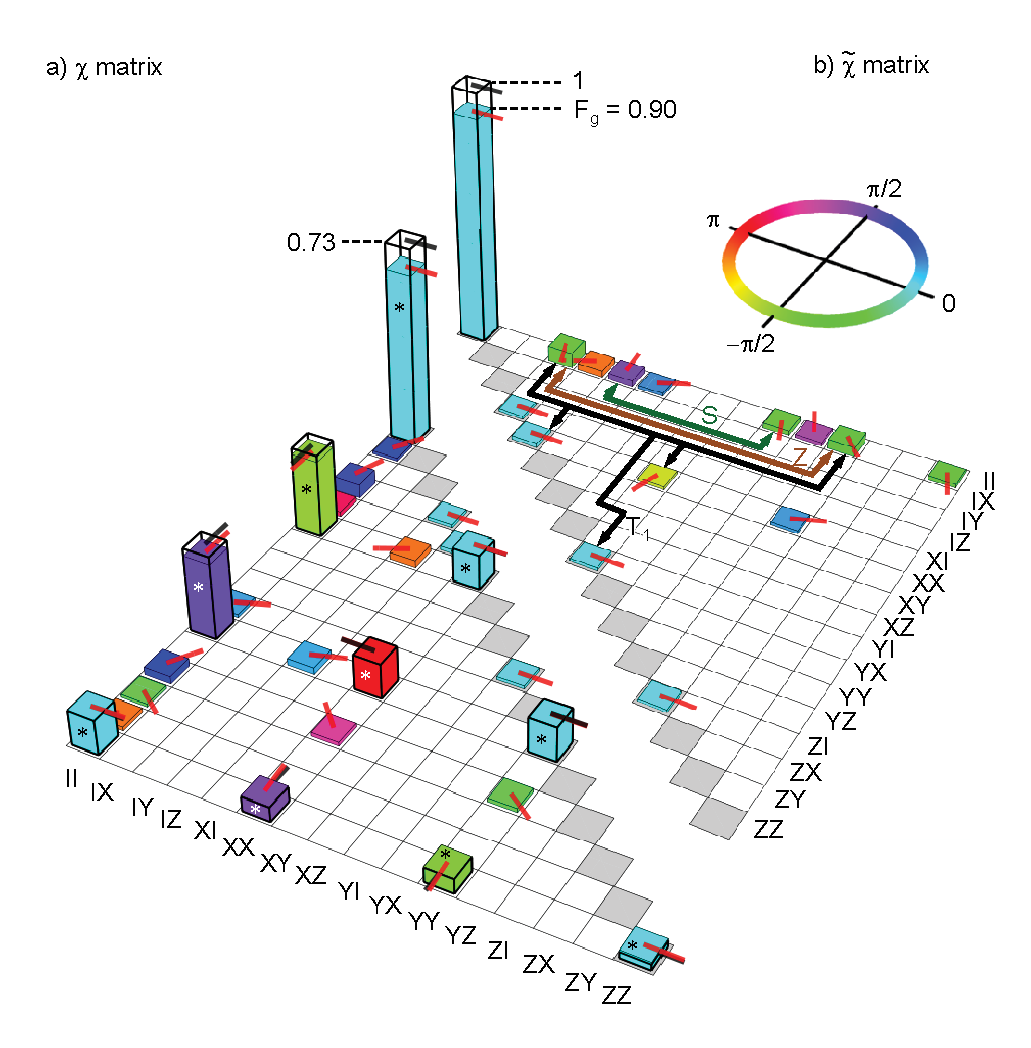
\includegraphics[width=1.\textwidth]{./material/papers/iswap/figures/chi_matrix_and_error_process}
	\label{fig:GateChiMatrixAndErrorProcess}
	\caption{}
\end{figure}


\section{Running Grover's Search Algorithm}

%Motivate this experiment:
% -Benchmark for superconducting quantum computers
% -Speed-up for searching in an unsorted database

\begin{figure}
	\centering
		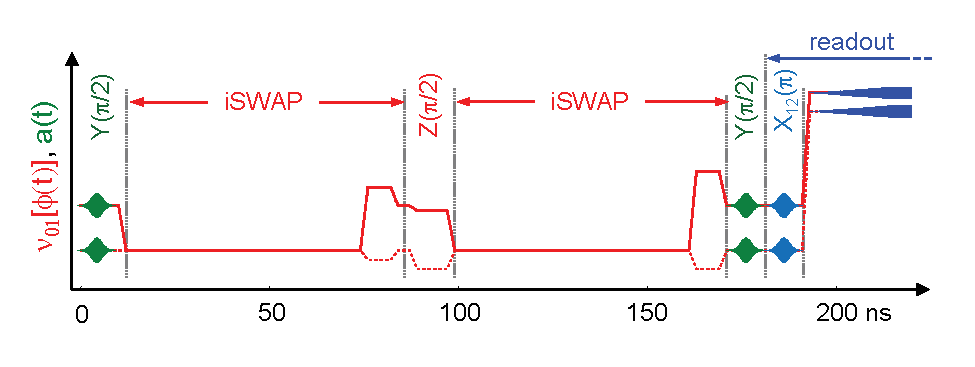
\includegraphics[width=1.\textwidth]{./material/papers/grover/figures/grover_algorithm_pulse_sequence}
	\label{fig:Grover3}
	\caption{The pulse sequence used in realizing Grover's quantum search algorithm. First, a $Y_{\pi/2}$ pulse is applied to each qubit to produce the fully superposed state $1/2(\ket{00}+\ket{01}+\ket{10}+\ket{11})$. Then, an $i\mathrm{SWAP}$ gate is applied, followed by a $Z_{\pm \pi /2}$ gate on each qubit, which corrsponds to the application of the oracle function. The resulting state is then analyzed using another $i\mathrm{SWAP}$ gate and two $Y_{\pi/2}$ gates to extract the state which has been marked by the oracle function. Optionally, a $Y^{12}_{\pi}$ pulse is used on each qubit to increase the readout fidelity.}
\end{figure}

\subsection{Introduction \& Motivation}

\begin{enumerate}
  \item {\textbf Inputs:} An oracle function $\mathcal{O}$ which performs the operation $O\ket{x}\ket{q} = \ket{x}\ket{q\otimes f(x)}$, where $f(x) = \delta_{x,x_0}$
  \item {\textbf Outputs:} The marked state $x_0$
	\item Initialize the qubit register to the state: 
	$$\ket{\psi} \to \ket{0}^{\otimes n}\ket{0}$$
	\item Apply the Hadamard transformation to all of the qubits: 
	$$\ket{psi}\to \frac{1}{\sqrt{2^n}}\sum\limits_{x=0}^{2^n-1} \ket{x} \left[ \frac{\ket{0}-\ket{1}}{\sqrt{2}} \right]$$
	\item Apply the Grover iteration $R \approx [\pi \sqrt{2^n}/4]$ times:
	$$ \ket{\psi} \to \left[(2 \ket{\psi}\bra{\psi}-I)\mathcal{O}\right]^R \frac{1}{\sqrt{2^n}} \sum\limits_{x=0}^{2^n-1}\ket{x} \left[ \frac{\ket{0}-\ket{1}}{\sqrt{2}} \right] \approx \ket{x_0}\left[\frac{\ket{0}-\ket{1}}{\sqrt{2}}\right] $$
	\item Measure the first n qubits to obtain $x_0$
\end{enumerate}

For the 2-qubit case, this algorithm can be drastically simplified -- or ``compiled'' -- such that it runs without the ancilla qubit and in one single step of the Grover iteration:

\begin{enumerate}
  \item {\textbf Inputs:} An oracle function $\mathcal{O}$ which performs the operation $O\ket{x} =(-1)^{\delta_{x,x_0}}\ket{x}$, where $x_0$ is the marked state that is searched.
  \item {\textbf Outputs:} The marked state $x_0$
	\item 
\end{enumerate}

%-Explain the Grover experiment...
%		-Theoretical interest
%		-First demonstration in NMR
%   -Potential speed-up
%   -Details of the algorithm:
%     -Elementary operations
%     -Pulse shapes, corrections, ...

\begin{figure}
	\centering
		\includegraphics[width=1.\textwidth]{./material/papers/grover/figures/grover_algorithm_schematic}
	\label{fig:GroverAlgorithmSchematic}
	\caption{}
\end{figure}

\subsection{Experimental Implementation}

%-Show the implementation principle of the experiment.
%  -Break down the algorithm using the universal quantum gates that we've implemented

\subsection{Results}

%To Do:
%  -Create figures for all steps of the algorithm using Matplotlib
%  -Re-Analyze the data using Denis' Mathematica
%-Discuss the results and errors.

\begin{figure}
	\centering
		\includegraphics[width=1.\textwidth]{./material/papers/grover/figures/grover_algorithm_experimental_results}
	\label{fig:GroverAlgorithmExperimentalResults}
	\caption{}
\end{figure}

\subsection{Conclusions}

%-Conclusions regarding quantum speed-up and applicability of results to larger-scale quantum computing.


\input{"scalable architecture"}

\chapter{Perspective \& Future Directions}

In chapters \ref{chapter:processor_characterization} and \ref{chapter:grover_algorithm} we demonstrated a universal two-qubit gate on our quantum processor and used it to realize the two-qubit Grover search algorithm, achieving probabilistic quantum speed-up. However, this approach to quantum computing cannot be scaled beyond a few qubits, wich is mostly due to the nature of the qubit-qubit coupling that has been chosen: The direct capacitive coupling produces a qubit-qubit interaction which is always on and whose amplitude decreases as $g_{qq}/\Delta_{qq}$. To be able to realize gate times which are shorter than the typical coherence time of Transmon qubits (typically $T_1,T_\phi \simeq\ 1-10 \;\mathrm{\mu s}$) we require coupling strengts $g_{qq}/2\pi \ge 10\;\mathrm{MHz}$. Therefore, in order to switch of spurious coupling between any two qubits below the 5 \% level, a detuning of $\Delta_{qq}\ge 20g \simeq 200\;\mathrm{MHz}$. For a processor where one would couple a large number of qubits using this scheme, the required qubit-qubit detunings would quickly lead to so-called {\it frequency crowding}, i.e. a shortage of available working point frequencies for the different qubits of the processor.

\smallskip

Hence, for a larger-scale quantum processor, it is essential to devise a coupling scheme which allows to deterministically turn on and off the coupling between arbitary qubits. In the literature, several architectures have been proposed for this, using e.g. a parametric coupling between qubits \citep{bertet_parametric_2006} or relying on the storage of quantum information stored in the qubits in a seperate entity, such as a superconducting resonator \citep{galiautdinov_resonatorzero-qubit_2012,mariantoni_implementing_2011}.

\smallskip

In the following section, we will propose a different approach to scalable quantum computing, based on a recently introduced double Transmon qubit \citep{srinivasan_tunable_2011} and using a fixed-frequency, microwave-tunable qubit-qubit coupling scheme as well as a single-shot readout method for individual qubits.

\smallskip

After shortly discussing our proposed architecture, we discuss recent developments in superconducting quantum computing and put them in context with our work, indicating possible future research directions.

\section{Designing a Scalable Architecture for Quantum Bits} \label{section:scalable_architecture}

In this section we describe our proposal for a scalable multi-qubit architecture based on superconducting Transmon qubits and fulfilling all of DiVincenzo's criteria for the realization of a quantum computer, as discussed in section \ref{section:divincenzo_criteria}. \citep{steane_how_2007}

\subsection{Requirements}

A scalable architecture for quantum computing should fulfill all criteria discussed above and, in addition do not incur an exponential experimental overhead for each qubit that is added to the quantum computer \citep{blume-kohout_climbing_2002}. Today, the two issues that are not addressed well by current qubit architectures, such as the quantum bus architecture used by many groups today \citep{dicarlo_demonstration_2009,wallraff_strong_2004}, which concern the qubit-qubit coupling and the readout of individual qubits. The quantum bus architecture, for instance, has an always-on coupling scheme between the qubits described by eq. (\ref{eq:cqed_bus_coupling}) which makes it hard to precisely control the coupling between individual qubits if a large number of them is present. Also, the readout of the qubit register is usually performed as a joint readout of the whole qubit register, thereby not allowing the read out of individual qubits.

\subsection{Qubit Parameters}

\begin{SCfigure}[1.0][ht!]
	\centering
	\includegraphics[width=0.35\textwidth]{./material/figures/scalable-architecture/qubit_molecule}
	\caption[...]{...}
	\label{fig:qubit_molecule_energies}
\end{SCfigure}

%
\begin{eqnarray}
\hat{H}_{dt}       & = & \hat{H}_q+\hat{H}_{qq} \\
\hat{H}_{q}/\hbar  & = & \omega_{01}^I\hat{\sigma}_z^I+\omega_{01}^{II}\hat{\sigma}_z^{II} \\
\hat{H}_{qq}/\hbar & = & g_{qq}\left(\hat{\sigma}_+^I\hat{\sigma}_-^{II}+\hat{\sigma}_-^I\hat{\sigma}_+^{II}\right) \\
\end{eqnarray}
%
We can rewrite $\hat{H}_{qq}$ in the eigenbasis $\ket{00}$, $\ket{01}$, $\ket{10}$, $\ket{11}$ of $\hat{H}_q$ as
%
\begin{equation}
\hat{H}_{qq}/\hbar = g_{qq}\left(\ket{10}\bra{01}+\ket{01}\bra{10}\right)
\end{equation}
%
When taking into account the second Transmon level $\ket{2}$, the capacitive coupling induces additional coupling elements
%
\begin{eqnarray}
\hat{H}_{qq}'/\hbar g_{qq} &  = &  \left(\ket{10}\bra{01}+\ket{01}\bra{10}\right) \\
& + & \sqrt{2}\left(\ket{11}\bra{02}+\ket{02}\bra{11}\right) \\
& + & \sqrt{2}\left(\ket{11}\bra{20}+\ket{20}\ket{11}\right) \\
& + & 2\left(\ket{21}\bra{12}+\ket{12}\bra{21}\right)
\end{eqnarray}
%
\subsection{Qubit-Qubit Coupling}

We couple the double Transmon to the resonator as shown in fig. \ref{fig:double_transmon_schematic} such that each of the two Transmons couples to the resonator with the same constant $g_{01}$. The resulting Hamiltonian, in analogy to Hamiltonian (\ref{eq:cqed_bus_coupling}) is
%
\begin{equation}
\hat{H}_{qr}/\hbar = g_{01}^I\left(\hat{\sigma}_+^I\hat{a}+\hat{\sigma}_-^I\hat{a}^\dagger\right)+g_{01}^{II}\left(\hat{\sigma}_+^{II}\hat{a}+\hat{\sigma}_-^{II}\hat{a}^\dagger \right), \label{eq:double_transmon_resonator_coupling}
\end{equation}
%
where, as before, the Hamiltonian of the resonator is given by eq. (\ref{eq:lc_hamiltonian}). As can be seen, the coupling operator between the two qubits and the resonator contains the sums $\hat{\sigma}_+^{I+II}=\hat{\sigma}_+^I+\hat{\sigma}_-^{II}$ and $\hat{\sigma}_-^{I+II}=\hat{\sigma}_-^I+\hat{\sigma}_-^{II}$. The eigenstates of $\hat{H}_{dt}$ at resonance $\omega_{01}^I)\omega_{01}^{II}$ are given as $\ket{00}$,$\ket{11}$, $\ket{\psi_+}=1/\sqrt{2}(\ket{01}+\ket{10})$ and $\ket{\psi_-}=1/\sqrt{2}(\ket{01}-\ket{10})$. Writing the Hamiltonian (\ref{eq:double_transmon_resonator_coupling}) in this eigenbasis yields
%
\begin{equation}
\hat{H}_{qr} = \sqrt{2}g_{01}\left[\left(\ket{11}\bra{\psi_+}+\ket{\psi_+}\bra{00}\right)\hat{a}+\left(\ket{\psi_+}\bra{11}+\ket{00}\bra{\psi_+}\right)\hat{a}^\dagger\right].
\end{equation}
%
As can be seen, the state $\ket{\psi_-}$ does not couple at all to the resonator, whereas the state $\ket{\psi_+}$ couples to it with an enhanced coupling rate $\sqrt{2}g_{01}$. The states $\ket{01}=(\ket{\psi_+}+\ket{\psi_-})/sqrt{2}$ and $\ket{10}=(\ket{\psi_+}-\ket{\psi_-})/\sqrt{2}$ couple to it at the normal rate $g_{01}$. Thus, if we operate the double Transmon at $\omega_{01}^I=\omega_{01}^{II}$ and ``park'' the qubit in the state $\ket{\psi_-}$, we can effectively switch off the coupling to the resonator. As proposed in \citep{srinivasan_tunable_2011}, we can peform an adiabatic passage $\ket{\psi_-}\to\ket{10}$ to switch on the qubit-resonator coupling of two or more qubits and perform a multi-qubit gate. Going back to the parking state $\ket{\psi_-}$ turns off the coupling again.

\subsection{Designing A Four-Qubit Architecture}

\begin{figure}[ht!]
	\centering
	\includegraphics[width=\textwidth]{./material/figures/scalable-architecture/qubit_architecture_energy_levels}
	\caption[]{}
	\label{fig:scalable_architecture_energy_levels}
\end{figure}

\subsection{Implementation}

\begin{figure}[ht!]
	\centering
	\includegraphics[width=\textwidth]{./material/figures/scalable-architecture/scalable_architecture_photos}
	\caption[]{}
	\label{fig:scalable_architecture_photos}
\end{figure}

\subsection{Scaling Up}

\section{Future Directions in Superconducting QC}

%-Discuss further developments in superconducting qc, such as:

\subsection{3D Circuit Quantum Electrodynamics}

%-Discuss the significance and potential of Q3CED

\subsection{Hybrid Quantum Systems}

%-Discuss hybrid quantum systems such as NV centers and their potential.
%  -Yui's & NTT NV center experiments
%  -Problems and possible solutions

\subsection{Quantum Error Correction \& Feedback}

%-Discuss quantum error correction.
%-Discuss quantum feedback.
%  -Siddiqi experiment, Yale paper
%  -Future directions taking into account the availability of highly coherent Transmon qubits


\appendix

\input{"appendix - modeling"}

\input{"appendix - data acquisition"}

\input{"appendix - fabrication"}

\bibliographystyle{apalike}

\stepcounter{chapter}

\addcontentsline{toc}{chapter}{\numberline {\thechapter} Bibliography}

\bibliography{thesis}

\end{document}
